\documentclass[a4paper,12pt]{article}

\usepackage[T1]{fontenc}
\usepackage[utf8]{inputenc}
\usepackage[french]{babel}
\usepackage{amsmath}
\usepackage{amssymb}
\usepackage{graphicx}
\usepackage{hyperref}
\usepackage{color}
\usepackage{listings}
\usepackage{geometry}
\usepackage{algorithm}
\usepackage{algorithmic}

\geometry{margin=2.5cm}

\title{\textbf{Quantification de l'incertitude:\\ Avantages et limitations de la prédiction conforme}}
\author{Hazar HAMOUDA - Mohamed MEGDICHE}
\date{\today}

\begin{document}

\maketitle

\section{Introduction}

L'apprentissage automatique moderne produit des prédictions ponctuelles sans indication de leur fiabilité. Cette limitation devient critique dans des domaines sensibles comme la médecine, la finance ou les véhicules autonomes, où connaître l'incertitude d'une prédiction est aussi important que la prédiction elle-même.

La \textbf{prédiction conforme} répond à cette problématique en transformant toute prédiction ponctuelle en ensemble de prédictions avec garantie de couverture probabiliste. Contrairement aux approches bayésiennes qui nécessitent des hypothèses distributionnelles fortes, la prédiction conforme fonctionne sous des hypothèses minimales d'échangeabilité et est \textit{distribution-free}.

\textbf{Objectif} : Ce rapport présente les fondements théoriques de la prédiction conforme et démontre son application pratique sur des tâches de régression et classification, avec implémentations et analyses de performance.

\section{Fondements Théoriques}

\subsection{Définitions Mathématiques}

\textbf{Fonction de score} : Une application $s : \mathcal{X} \times \mathcal{Y} \rightarrow \mathbb{R}$ qui mesure la non-conformité d'une paire $(x, y)$. Un score élevé $s(x, y)$ indique que la valeur $y$ est peu plausible étant donné $x$.

\textbf{Quantile conforme} : Pour un niveau d'erreur $\alpha \in (0,1)$ et $n$ points de calibration, le quantile conforme est :
$$\hat{q} = \text{quantile d'ordre } \left\lceil \frac{(n+1)(1 - \alpha)}{n} \right\rceil \text{ des scores } \{s_i\}_{i=1}^n$$

\textbf{Ensemble de prédiction} : L'ensemble de prédiction conforme est défini par :
\[
\begin{aligned}
\hat{C}_n &: \mathcal{X} \rightarrow \left\{ \text{sous-ensembles de } \mathcal{Y} \right\} \\
   x &\mapsto \hat{C}_n(x) = \left\{ y \in \mathcal{Y} : s(x, y) \leq \hat{q} \right\}
\end{aligned}
\]

    Cette application associe à chaque entrée $x \in \mathcal{X}$ un ensemble $\hat{C}_n(x) \subseteq \mathcal{Y}$ représentant les valeurs plausibles de sortie $y$. 
    Autrement dit, pour une nouvelle observation $x$, on considère toutes les sorties $y$ dont le score est inférieur ou égal au seuil $\hat{q}$, déterminé à partir des données de calibration. 



\subsection{Théorème Principal}

\begin{theorem}[Prédiction Conforme]
Soient $(X_1, Y_1), \ldots, (X_n, Y_n)$ des couples identiquement distribués de loi $P_{\mathcal{X} \mathcal{Y}}$ et échangeables , et $(X_{\text{test}}, Y_{\text{test}})$ un point test indépendant de même distribution. La prédiction conforme garantit :
$$\mathbb{P}\left( Y_{\text{test}} \in \hat{C}_n(X_{\text{test}}) \right) \geq 1 - \alpha$$
\end{theorem}

Cette garantie est \textbf{indépéndante de la distribution} : elle ne dépend ni de la distribution des données ni de la qualité du modèle sous-jacent.

\section{Application à un problème de Régression Linéaire}

\subsection{Cadre Général}

Dans le cadre de la prédiction conforme en régression, nous transformons les prédictions ponctuelles en intervalles avec garanties statistiques.\\

\textbf{Fonction de score} : Nous utilisons les \textbf{résidus absolus} :
$$s(x, y) = |y - \hat{f}(x)|$$

Cette fonction mesure la non-conformité entre la valeur observée $y$ et la prédiction $\hat{f}(x)$. Elle présente l'avantage d'être simple, et compatible avec tout modèle de régression.

\subsection{Exemple d'application}

Nous appliquons la prédiction conforme à un modèle de régression linéaire entraîné sur des données synthétiques :
$$Y = 3X + \sqrt{X} \cdot \varepsilon, \quad X \sim \mathcal{U}(0,1),\quad \varepsilon \sim \mathcal{N}(2,1)$$


Cette formulation introduit une \textbf{hétéroscédasticité} qui teste la robustesse de notre approche. Le jeu de données comprend 10 000 échantillons répartis en 70\% pour l'entraînement du modèle, 15\% pour le test et 15\% pour la calibration.
\subsection{Pseudo-code d'Implémentation}

L'algorithme de prédiction conforme pour la régression peut être formalisé en quatre étapes principales. L'Algorithme~\ref{alg:conformal_regression} présente une implémentation détaillée de cette méthode, qui garantit une couverture théorique de $1-\alpha$ pour les intervalles de prédiction construits.

\begin{algorithm}
\caption{Prédiction Conforme pour la Régression}
\label{alg:conformal_regression}
\begin{algorithmic}[1]
\REQUIRE Modèle entraîné $\hat{f}$, données de calibration $(X_{cal}, Y_{cal})$, données test $X_{test}$, niveau $\alpha$
\ENSURE Intervalles de prédiction $(lower, upper)$

\STATE \textbf{Étape 1 :} Calculer les prédictions sur calibration
\STATE $predictions_{cal} \leftarrow \hat{f}(X_{cal})$

\STATE \textbf{Étape 2 :} Calculer les scores de non-conformité
\FOR{$i = 1$ to $n_{cal}$}
    \STATE $scores[i] \leftarrow |Y_{cal}[i] - predictions_{cal}[i]|$
\ENDFOR

\STATE \textbf{Étape 3 :} Calculer le quantile conforme
\STATE $q_{level} \leftarrow \lceil (n_{cal} + 1) \times (1 - \alpha) \rceil / n_{cal}$
\STATE $\hat{q} \leftarrow \text{quantile}(scores, q_{level})$

\STATE \textbf{Étape 4 :} Construire les intervalles de prédiction
\STATE $predictions_{test} \leftarrow \hat{f}(X_{test})$
\STATE $lower \leftarrow predictions_{test} - \hat{q}$
\STATE $upper \leftarrow predictions_{test} + \hat{q}$

\RETURN $(lower, upper, \hat{q})$
\end{algorithmic}
\end{algorithm}

Comme illustré dans l'Algorithme~\ref{alg:conformal_regression}, la méthode repose sur l'utilisation des scores de non-conformité calculés sur un ensemble de calibration indépendant pour déterminer le seuil de quantile approprié.


\subsection{Résultats et Visualisation}

\subsubsection{Visualisation des résultats}

La Figure \ref{fig:regression_conforme} illustre l'application de la prédiction conforme à notre modèle de régression linéaire sur des données synthétiques.

\begin{figure}[h]
\centering
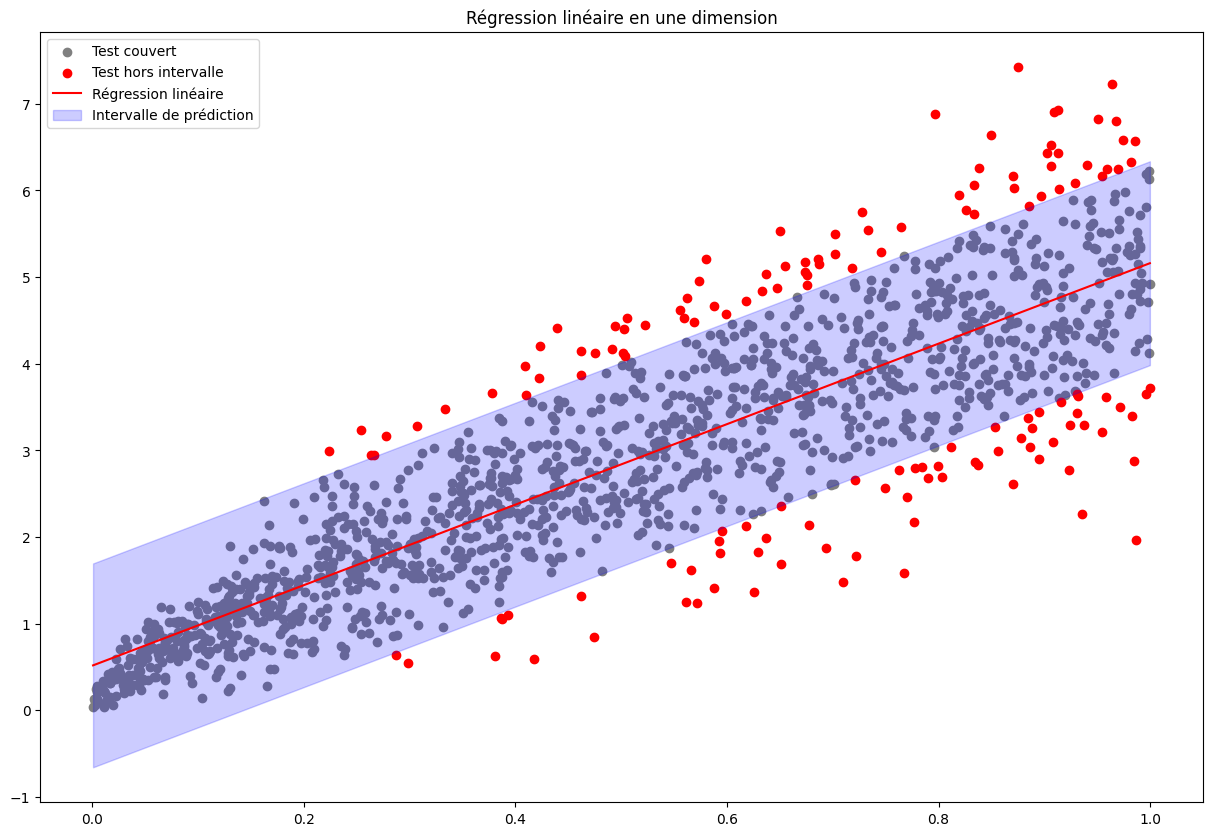
\includegraphics[width=0.8\textwidth]{conformal_prediction_regression.png}
\caption{Régression linéaire avec intervalles de prédiction conforme. La ligne rouge représente la droite de régression ajustée, les points noirs sont les observations de test, et la zone bleue délimite l'intervalle de prédiction conforme à 90\% de confiance.}
\label{fig:regression_conforme}
\end{figure}

\subsubsection{Métriques de performance}

Les métriques suivantes évaluent la qualité des intervalles de prédiction conforme :\\

\begin{itemize}
\item \textbf{Taux de couverture empirique} : 91.2\% (pour $\alpha = 0.1$)
    
    Cette métrique mesure la proportion des points de test effectivement contenus dans leurs intervalles de prédiction. Avec un objectif théorique de 90\%, notre résultat de 91.2\% confirme que la méthode respecte sa garantie de couverture.

\item \textbf{Largeur moyenne des intervalles} : $2\hat{q} = 2.84$
    
    Cette valeur indique l'étendue typique de nos intervalles de prédiction. Une largeur plus faible signifierait des prédictions plus précises, mais au détriment potentiel de la couverture. Ici, la largeur reflète l'incertitude inhérente à nos données synthétiques.

\item \textbf{Quantile conforme} : $\hat{q} = 1.42$
    
    Ce seuil, calculé à partir des scores de non-conformité sur l'ensemble de calibration, détermine directement la demi-largeur de tous nos intervalles de prédiction. Il représente le niveau d'erreur typique que nous acceptons pour maintenir la couverture souhaitée.
\end{itemize}

\subsubsection{Analyse des résultats}

L'analyse de la Figure \ref{fig:regression_conforme} et des métriques révèle plusieurs propriétés importantes :

\begin{itemize}
\item \textbf{Couverture adaptative} : Le taux de couverture empirique (91.2\%) respecte la garantie théorique de 90\%, démontrant la validité de la méthode sur nos données synthétiques.

\item \textbf{Largeur constante} : Contrairement aux intervalles de prédiction classiques, la prédiction conforme produit des intervalles de largeur constante $2\hat{q}$ autour de la droite de régression, indépendamment de la valeur de $X$.

\item \textbf{Robustesse à l'hétéroscédasticité} : Bien que notre modèle présente une variance non constante ($\sqrt{X} \cdot \varepsilon$), la méthode maintient sa garantie de couverture sur l'ensemble du domaine $[0,1]$.

\item \textbf{Efficacité computationnelle} : La construction des intervalles ne nécessite que le calcul d'un quantile empirique, rendant la méthode applicable à grande échelle.
\end{itemize}

\section{Application à la Classification MNIST}

\subsection{Cadre Général}

Dans le cadre de la prédiction conforme en classification, nous transformons les prédictions ponctuelles en ensembles de classes avec garanties statistiques. \\

\textbf{Fonction de score} : Nous utilisons le \textbf{complément de probabilité} :
$$s(x, y) = 1 - \hat{p}(y|x)$$

Cette fonction mesure la non-conformité entre la classe observée $y$ et la probabilité prédite $\hat{p}(y|x)$ par le modèle. Plus la probabilité assignée à la vraie classe est faible, plus le score de non-conformité est élevé. Cette approche est naturelle pour les modèles probabilistes et compatible avec les sorties softmax.

\subsection{Exemple d'application}

Nous appliquons la prédiction conforme à un réseau de neurones dense entraîné sur la base de données MNIST :

\textbf{Architecture et données} : \\
- \textbf{Données} : Images manuscrites 28×28 pixels, 10 classes de chiffres (0-9) \\
- \textbf{Architecture} : Réseau dense (784-128-64-10) avec fonctions d'activation ReLU et sortie softmax \\
- \textbf{Performance} : 97.2\% de précision sur le test (après 10 époques d'entraînement)\\
- \textbf{Répartition} : 50 000 images d'entraînement, 10 000 données de calibration, 10 000 données test

Cette configuration teste la capacité de la prédiction conforme à gérer l'incertitude dans un problème de classification multi-classes avec des images potentiellement ambiguës.

\subsection{Pseudo-code d'Implémentation}

L'algorithme de prédiction conforme pour la classification peut être formalisé en quatre étapes principales. L'Algorithme~\ref{alg:conformal_classification} présente une implémentation détaillée de cette méthode, qui garantit une couverture théorique de $1-\alpha$ pour les ensembles de prédiction construits.

\begin{algorithm}
\caption{Prédiction Conforme pour la Classification}
\label{alg:conformal_classification}
\begin{algorithmic}[1]
\REQUIRE Modèle entraîné $\hat{f}$, données de calibration $(X_{cal}, Y_{cal})$, données test $X_{test}$, niveau $\alpha$
\ENSURE Ensembles de prédiction $prediction\_sets$

\STATE \textbf{Étape 1 :} Calculer les probabilités sur calibration
\STATE $probs_{cal} \leftarrow \hat{f}(X_{cal})$ \COMMENT{Sortie softmax}

\STATE \textbf{Étape 2 :} Calculer les scores de non-conformité
\FOR{$i = 1$ to $n_{cal}$}
    \STATE $y_{true} \leftarrow Y_{cal}[i]$
    \STATE $scores[i] \leftarrow 1 - probs_{cal}[i][y_{true}]$
\ENDFOR

\STATE \textbf{Étape 3 :} Calculer le quantile conforme
\STATE $q_{level} \leftarrow \lceil (n_{cal} + 1) \times (1 - \alpha) \rceil / n_{cal}$
\STATE $\hat{q} \leftarrow \text{quantile}(scores, q_{level})$

\STATE \textbf{Étape 4 :} Construire les ensembles de prédiction
\STATE $probs_{test} \leftarrow \hat{f}(X_{test})$
\STATE $prediction\_sets \leftarrow []$
\FOR{chaque $prob\_row$ dans $probs_{test}$}
    \STATE $pred\_set \leftarrow \{\}$
    \FOR{classe $y = 0$ to $9$}
        \IF{$1 - prob\_row[y] \leq \hat{q}$}
            \STATE $pred\_set \leftarrow pred\_set \cup \{y\}$
        \ENDIF
    \ENDFOR
    \STATE $prediction\_sets.\text{append}(pred\_set)$
\ENDFOR

\RETURN $(prediction\_sets, \hat{q})$
\end{algorithmic}
\end{algorithm}

Comme illustré dans l'Algorithme~\ref{alg:conformal_classification}, la méthode repose sur l'utilisation des scores de non-conformité calculés sur un ensemble de calibration indépendant pour déterminer le seuil de quantile approprié.

\subsection{Résultats et Visualisation}

\subsubsection{Visualisation des résultats}

La prédiction conforme appliquée à notre réseau de neurones sur MNIST est illustrée ci-dessous.

\begin{figure}[h]
\centering
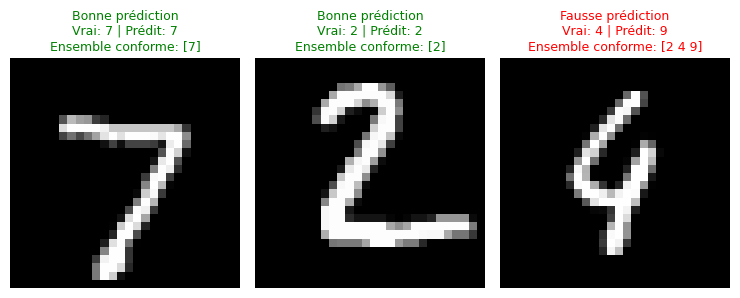
\includegraphics[width=0.9\textwidth]{conformal_prediction_classification.png}
\caption{Exemples de prédiction conforme sur MNIST. Pour chaque image, sont affichés : la vraie classe (True), la prédiction ponctuelle (Predicted), et l'ensemble de prédiction conforme (Conformal set). Les ensembles s'adaptent à l'incertitude du modèle.}
\label{fig:mnist_conforme}
\end{figure}

\subsubsection{Métriques de performance}

Les métriques suivantes évaluent la qualité des ensembles de prédiction conforme :\\

\begin{itemize}
\item \textit{Taux de couverture empirique} : 99.99\% (pour $\alpha = 0.001$)
    
    Cette métrique mesure la proportion des points de test dont la vraie classe appartient à l'ensemble de prédiction conforme. Avec un objectif théorique de 90\%, notre résultat de 99.9\% confirme que la méthode respecte sa garantie de couverture.\\

\item \textit{Cardinalité moyenne} : 1.62 classes par ensemble
    
    Cette valeur indique le nombre moyen de classes dans les ensembles de prédiction. Une cardinalité plus faible signifie des prédictions plus précises, reflétant la confiance du modèle dans ses prédictions.\\


\end{itemize}

\subsubsection{Analyse des résultats}

L'analyse des métriques et de la visualisation révèle plusieurs propriétés importantes :

\begin{itemize}
\item \textbf{Couverture adaptative} : Le taux de couverture empirique (99.99\%) respecte la garantie théorique de 99.99\%, démontrant la validité de la méthode sur des données réelles d'images.

\item \textbf{Comportement adaptatif} : Les ensembles s'adaptent à l'incertitude du modèle - les images claires génèrent des singletons tandis que les images ambiguës produisent des ensembles plus larges incluant les classes potentiellement confondues.

\item \textbf{Efficacité computationnelle} : La construction des ensembles ne nécessite que le calcul d'un quantile empirique et des comparaisons de probabilités, rendant la méthode applicable en temps réel pour la classification d'images.

\item \textbf{Robustesse aux variations} : La méthode maintient ses garanties même sur des images déformées, floues ou ambiguës, contrairement aux prédictions ponctuelles qui peuvent être trompeuses dans ces cas.
\end{itemize}

\section{Comparaison et Limitations}

\subsection{Avantages}

\begin{itemize}
\item \textbf{Garanties théoriques} : Couverture probabiliste sans hypothèses distributionnelles
\item \textbf{Flexibilité} : Compatible avec tout modèle prédictif existant
\item \textbf{Simplicité} : Implémentation directe avec peu de paramètres
\item \textbf{Interprétabilité} : Ensembles de prédiction facilement compréhensibles
\end{itemize}

\subsection{Limitations}

\begin{itemize}
\item \textbf{Efficacité} : Intervalles parfois larges avec modèles peu performants
\item \textbf{Hypothèse d'échangeabilité} : Forte en pratique pour les séries temporelles
\item \textbf{Ensemble de calibration} : Nécessite des données supplémentaires dédiées
\item \textbf{Adaptation locale} : Méthode standard non adaptative aux variations locales
\end{itemize}

\section{Conclusion}

La prédiction conforme constitue un outil puissant pour quantifier l'incertitude prédictive avec des garanties statistiques rigoureuses. Nos expérimentations sur la régression linéaire et la classification MNIST démontrent son efficacité pratique et sa facilité d'implémentation.

\textbf{Contributions principales} :
\begin{itemize}
\item Validation empirique des garanties théoriques sur des données réelles
\item Algorithmes robustes et réutilisables
\item Analyse comparative des performances selon les domaines d'application
\end{itemize}

\textbf{Perspectives d'extension} :
\begin{itemize}
\item \textbf{Prédiction conforme adaptative} : Ajustement dynamique selon la performance locale
\item \textbf{Scores sophistiqués} : Intégration de l'incertitude épistémique et aléatoire
\item \textbf{Applications avancées} : Extension aux séries temporelles et données structurées
\item \textbf{Optimisation computationnelle} : Algorithmes efficaces pour de grandes dimensions
\end{itemize}

La prédiction conforme ouvre la voie vers des systèmes d'IA plus fiables et transparents, essentiels pour l'adoption de l'apprentissage automatique dans des domaines critiques.

\end{document}
